\documentclass{standalone}
\usepackage{pgfplots}
\pgfplotsset{compat=1.16}
\begin{document}
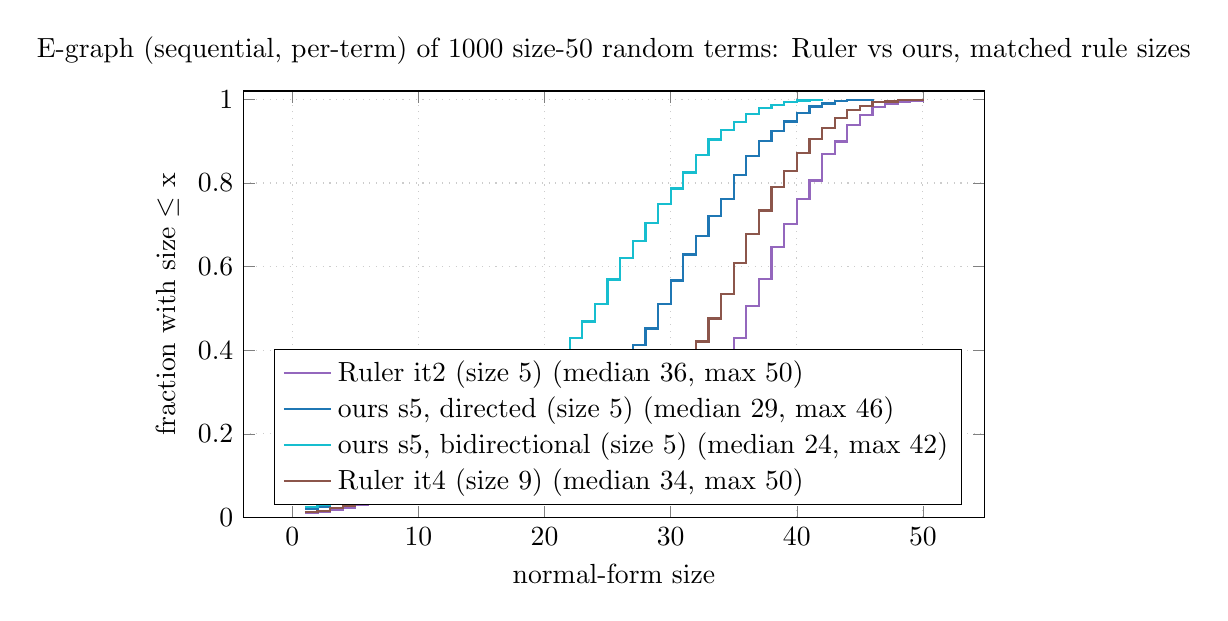
\begin{tikzpicture}
  \begin{axis}[
      width=11cm, height=7cm,
      xlabel={normal-form size}, ylabel={fraction with size $\leq$ x},
      title={E-graph (sequential, per-term) of 1000 size-50 random terms: Ruler vs ours, matched rule sizes},
      ymin=0, ymax=1.02, grid=both, grid style={dotted, gray!40},
      legend pos=south east, legend cell align=left,]
    \definecolor{c0}{HTML}{9467bd}
    \addplot[color=c0, thick, const plot] coordinates {(1,0.0120) (2,0.0130) (3,0.0190) (4,0.0230) (5,0.0300) (6,0.0350) (7,0.0390) (8,0.0470) (9,0.0490) (10,0.0560) (11,0.0600) (12,0.0650) (13,0.0680) (14,0.0710) (15,0.0810) (16,0.0860) (17,0.0900) (18,0.0970) (19,0.1080) (20,0.1150) (21,0.1190) (22,0.1250) (23,0.1330) (24,0.1410) (25,0.1540) (26,0.1650) (27,0.1810) (28,0.1980) (29,0.2080) (30,0.2300) (31,0.2520) (32,0.2910) (33,0.3340) (34,0.3720) (35,0.4300) (36,0.5050) (37,0.5700) (38,0.6460) (39,0.7020) (40,0.7610) (41,0.8060) (42,0.8690) (43,0.8990) (44,0.9390) (45,0.9630) (46,0.9820) (47,0.9880) (48,0.9930) (49,0.9960) (50,1.0000)};
    \addlegendentry{Ruler it2 (size 5) (median 36, max 50)}
    \definecolor{c1}{HTML}{1f77b4}
    \addplot[color=c1, thick, const plot] coordinates {(1,0.0210) (2,0.0250) (3,0.0400) (4,0.0520) (5,0.0600) (6,0.0760) (7,0.0830) (8,0.0940) (9,0.1010) (10,0.1110) (11,0.1210) (12,0.1310) (13,0.1420) (14,0.1520) (15,0.1620) (16,0.1680) (17,0.1760) (18,0.1880) (19,0.2080) (20,0.2200) (21,0.2400) (22,0.2560) (23,0.2880) (24,0.3150) (25,0.3450) (26,0.3790) (27,0.4130) (28,0.4520) (29,0.5110) (30,0.5670) (31,0.6290) (32,0.6730) (33,0.7210) (34,0.7610) (35,0.8190) (36,0.8640) (37,0.9000) (38,0.9250) (39,0.9470) (40,0.9680) (41,0.9830) (42,0.9900) (43,0.9960) (44,0.9980) (45,0.9990) (46,1.0000)};
    \addlegendentry{ours s5, directed (size 5) (median 29, max 46)}
    \definecolor{c2}{HTML}{17becf}
    \addplot[color=c2, thick, const plot] coordinates {(1,0.0260) (2,0.0310) (3,0.0590) (4,0.0830) (5,0.0970) (6,0.1230) (7,0.1320) (8,0.1440) (9,0.1520) (10,0.1700) (11,0.1830) (12,0.1980) (13,0.2070) (14,0.2240) (15,0.2470) (16,0.2620) (17,0.2890) (18,0.3150) (19,0.3460) (20,0.3710) (21,0.3930) (22,0.4300) (23,0.4690) (24,0.5110) (25,0.5690) (26,0.6200) (27,0.6620) (28,0.7040) (29,0.7490) (30,0.7870) (31,0.8250) (32,0.8660) (33,0.9040) (34,0.9270) (35,0.9450) (36,0.9650) (37,0.9790) (38,0.9860) (39,0.9930) (40,0.9970) (41,0.9990) (42,1.0000)};
    \addlegendentry{ours s5, bidirectional (size 5) (median 24, max 42)}
    \definecolor{c3}{HTML}{8c564b}
    \addplot[color=c3, thick, const plot] coordinates {(1,0.0130) (2,0.0160) (3,0.0230) (4,0.0280) (5,0.0340) (6,0.0410) (7,0.0440) (8,0.0520) (9,0.0590) (10,0.0670) (11,0.0730) (12,0.0760) (13,0.0780) (14,0.0850) (15,0.1000) (16,0.1060) (17,0.1110) (18,0.1220) (19,0.1360) (20,0.1430) (21,0.1490) (22,0.1570) (23,0.1660) (24,0.1770) (25,0.1950) (26,0.2180) (27,0.2450) (28,0.2620) (29,0.2880) (30,0.3270) (31,0.3650) (32,0.4210) (33,0.4760) (34,0.5350) (35,0.6090) (36,0.6780) (37,0.7340) (38,0.7910) (39,0.8290) (40,0.8720) (41,0.9050) (42,0.9310) (43,0.9550) (44,0.9750) (45,0.9840) (46,0.9930) (47,0.9950) (48,0.9980) (49,0.9990) (50,1.0000)};
    \addlegendentry{Ruler it4 (size 9) (median 34, max 50)}
  \end{axis}
\end{tikzpicture}
\end{document}
